% Plain-language version. Same work, same numbers, written for a reader who does not work on
% speech anti-spoofing. Build: pdflatex main_plain && bibtex main_plain && pdflatex main_plain x2
\documentclass[11pt,a4paper]{article}

\usepackage[margin=1in]{geometry}
\usepackage{graphicx}
\usepackage{booktabs}
\usepackage{amsmath}
\usepackage{caption}
\usepackage{microtype}
\usepackage{xcolor}
\usepackage[hidelinks]{hyperref}
\usepackage{natbib}

\captionsetup{font=small,labelfont=bf,skip=6pt}
\newcommand{\best}[1]{\textbf{#1}}

\title{\bf Four Detectors That Turned Out to Be One:\\
What We Learned Trying to Catch Fake Speech}

\author{A.\ Harisha\\[2pt]
\small Sahyadri College of Engineering and Management\\
\small \texttt{harisha@sahyadri.edu.in}}

\date{\today}

\begin{document}
\maketitle

\begin{abstract}
\noindent
Software can now generate speech that sounds like a real person, so we need software that can tell
real speech from fake. The usual way to build a strong detector is to build several different ones
and average their answers, hoping their mistakes differ. We built four detectors that were different
by design, and found they made almost the same mistakes: together they were worth about one
detector, not four. We also found that the standard way of choosing which detector to use does not
work on this data, and that the detector which scores best on the official test is the one that
performs worst on real audio collected from the internet. Our best honestly-chosen system gets 3.21
out of 100 wrong at its break-even point, which is good but behind the best published system at
2.59.
\end{abstract}

\section{What this is about}

A computer can now be given a few seconds of someone's voice and produce new sentences in that
voice. This is useful for accessibility and dubbing, and harmful for fraud and impersonation. So
researchers build \emph{detectors}: programs that listen to a recording and output a number saying
how likely it is to be genuine.

\paragraph{How detectors are scored.} We mostly use one number, the \textbf{equal error rate}, or
EER. Imagine turning a dial on the detector. Turn it one way and it becomes suspicious, catching
every fake but also wrongly flagging real speech. Turn it the other way and it trusts everything,
never flagging real speech but missing fakes. Somewhere in the middle, the two kinds of mistake
happen equally often. That percentage is the EER. \textbf{Lower is better:} an EER of 3\% means that
at the balanced setting, three out of a hundred judgements are wrong. We also report a cost-weighted
score called minDCF, which penalises the more expensive mistake more heavily.

\paragraph{The data.} We use ASVspoof~5 \citep{asvspoof5}, the standard public benchmark. It has one
property that makes it honest: the fake-speech systems used in the training data are \emph{different}
from the ones in the test data. A detector cannot pass by memorising the particular fakes it was
shown. Table~\ref{tab:plain_data} describes it.

\begin{table}[t]
\centering
\small
\caption{The data we used. The fake-generation systems in each part do not overlap, so the test
always uses fakes the detector has never seen.}
\label{tab:plain_data}
\begin{tabular}{lrrl}
\toprule
Part & Recordings & Real speech & What it is for \\
\midrule
Training & 182{,}357 & 10\% & teaching the detector \\
Development & 140{,}950 & 22\% & choosing between detectors \\
Test & 680{,}774 & 20\% & the final score, used once \\
In-the-Wild & 31{,}779 & 63\% & audio from the internet, a reality check \\
\bottomrule
\end{tabular}
\end{table}

\section{What we built}

Every one of our detectors has the same two stages (Figure~\ref{fig:plain_arch}).

The \textbf{first stage} is a large pre-trained model called WavLM \citep{wavlm}. It was trained on
94{,}000 hours of ordinary speech, with no knowledge of fakes at all, and it turns a recording into a
rich numerical description. We barely change it; we attach a small number of extra parameters using a
technique called LoRA \citep{lora}, which lets us adjust a 300-million-parameter model by training
only about 3 million numbers.

The \textbf{second stage}, which we call the back-end, is a small network that reads that description
and produces the final score. This is the part we varied. We built four:

\begin{itemize}\itemsep3pt
\item \textbf{Pool} --- the ordinary approach. It averages the description over the whole recording,
then decides. Averaging over time throws away \emph{when} things happened.
\item \textbf{MHFA} --- instead of averaging, it learns \emph{where in the recording to look}.
\item \textbf{LFCC} --- it adds a completely separate description of the sound, a classical one
based on frequency content, computed directly from the waveform rather than from WavLM.
\item \textbf{Graph} --- it treats pieces of the recording as points in a network and lets them
exchange information, an idea borrowed from a detector called AASIST \citep{aasist}.
\end{itemize}

Everything else is held identical: same training data, same random seed, same schedule. So any
difference between them comes from the back-end alone.

\begin{figure}[t]
\centering
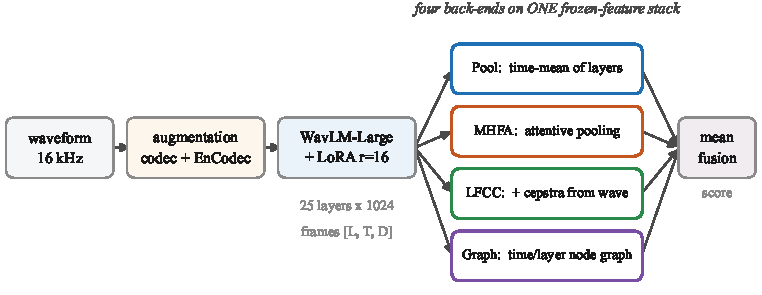
\includegraphics[width=\textwidth]{figures/fig1_architecture}
\caption{All four detectors share the first stage and differ only in the last box before the score.}
\label{fig:plain_arch}
\end{figure}

\section{Finding 1: the four detectors were really one detector}

The reason to build several detectors is that averaging helps \emph{only if they make different
mistakes}. If two detectors are wrong about exactly the same recordings, averaging them changes
nothing.

So we measured how different they actually were. Think of each detector's set of scores as a
direction. If the four directions point different ways, we have four detectors. If they all point
the same way, we have one.

The result is Figure~\ref{fig:plain_spectrum}. A single shared direction accounts for \best{95.5\%}
of everything the four detectors do, and all four contribute to it almost exactly equally. By a
standard measure of how many independent things are in a set, our four detectors are worth
\best{1.10}.

\begin{figure}[t]
\centering
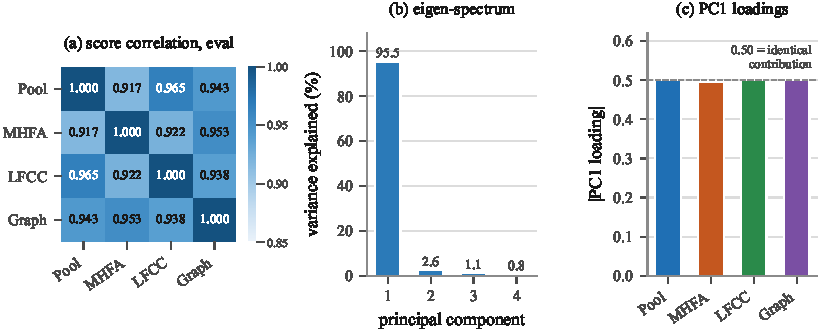
\includegraphics[width=\textwidth]{figures/fig6_spectrum}
\caption{(a) How similar the detectors' scores are --- 0.92 to 0.97, where 1.00 would mean
identical. (b) One shared direction explains 95.5\% of their behaviour. (c) All four contribute to
it equally.}
\label{fig:plain_spectrum}
\end{figure}

We changed the way the model summarises time, the kind of sound description it reads, the shape of
its network, and even the large pre-trained model underneath. All of that moved the count from 1.00
to 1.10.

The one change that helped at all was MHFA --- the detector that looks at \emph{when} things happen
instead of averaging them away. Averaging a four-second clip into a single summary turns out to
throw away more than we expected. That change bought a small but real improvement, and it came from
the 3\% of behaviour the detectors did \emph{not} share.

\section{Finding 2: we cannot tell which detector is best}

Standard practice is: train on part of the data, use a second part (the \emph{development} set) to
choose your best system, then report its score on the test set. Using the test set to choose would be
cheating, because then the score no longer predicts anything new.

We followed that rule. It did not work.

We had 15 possible combinations of our four detectors. We ranked them by their development score and
compared that to their test score. \textbf{The two rankings are unrelated} ---
Figure~\ref{fig:plain_select} shows the correlation is $+0.01$, which is statistically
indistinguishable from pure chance.

\begin{figure}[t]
\centering
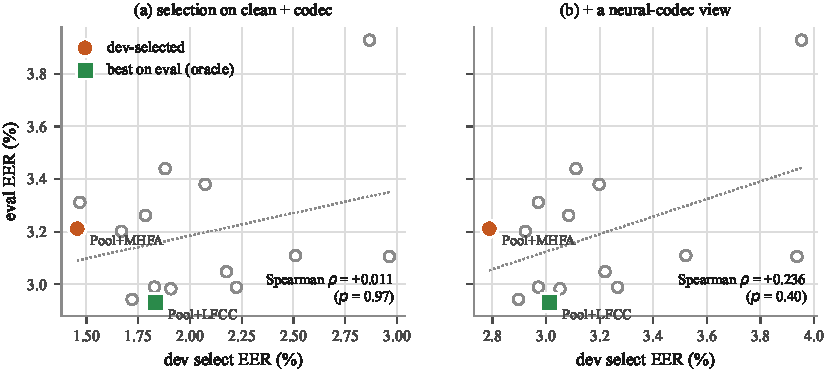
\includegraphics[width=\textwidth]{figures/fig7_selection}
\caption{Each dot is one combination of detectors. If the development set were useful, the dots
would fall along a rising line. They do not.}
\label{fig:plain_select}
\end{figure}

\paragraph{Why.} The training and development recordings are all clean, uncompressed audio. Three
quarters of the test recordings have been through a compression codec --- the kind of processing a
phone call or a voice message applies. So the development set simply never shows us the thing the
test set is actually judging.

We tried the obvious fix: we added compressed audio to the development set. The ranking improved,
but not enough; the correlation rose to $+0.24$, still within chance.

\paragraph{What it costs us, stated openly.} Our rule picks a system scoring \best{3.21}. The best
system we actually have scores \textbf{2.93}, and our rule ranks it seventh out of fifteen. We report
\textbf{both} numbers, in Table~\ref{tab:plain_results}, and we label the second one clearly as a
system we could not have chosen honestly. The 0.28 gap between them is not a flaw in our detectors.
It is a measurement of how poor the selection procedure is.

\begin{table}[t]
\centering
\small
\caption{Results on the test set. Lower is better. The oracle row is what we would have picked if we
were allowed to cheat by looking at the test set; we show it for honesty, not as our result.}
\label{tab:plain_results}
\begin{tabular}{llrr}
\toprule
System & How it was chosen & EER (\%) & minDCF \\
\midrule
Best published system, 12 detectors \citep{ustc2024} & --- & 2.59 & 0.0750 \\
Pool + LFCC & \emph{oracle --- not claimed} & \emph{2.93} & \emph{0.0819} \\
\best{Pool + MHFA} & \best{our rule} & \best{3.21} & \best{0.0905} \\
Pool alone & --- & 3.31 & 0.0942 \\
Another published system \citep{szuafs} & --- & 4.04 & 0.115 \\
\bottomrule
\end{tabular}
\end{table}

\section{Finding 3: doing well on the test says little about the real world}

The test set is large and carefully built, but every recording in it was made by one project under
controlled conditions. So we also ran our detectors on In-the-Wild: about 32{,}000 clips of real and
fake speech of public figures, collected from the internet, with no labels about how they were
recorded.

Two things happened (Figure~\ref{fig:plain_transfer}).

\textbf{Everything got much worse.} Error rates roughly tripled, from 3--4\% to 8--12\%. That is
normal in this field but rarely stated plainly.

\textbf{The order flipped.} LFCC, our \emph{best} detector on the official test, was our
\emph{worst} on internet audio. MHFA, which was third on the official test, was clearly the best in
the wild --- 8.51 against 11.25 for the next one.

\begin{figure}[t]
\centering
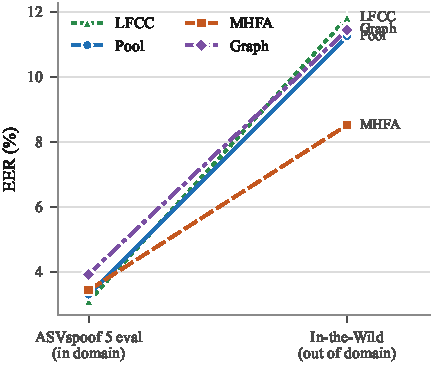
\includegraphics[width=\textwidth]{figures/fig8_transfer}
\caption{Each line is one detector, from the official test on the left to internet audio on the
right. The lines cross: the winner on the left is the loser on the right.}
\label{fig:plain_transfer}
\end{figure}

A likely explanation is that LFCC partly learned the \emph{recording conditions} of this particular
dataset rather than what makes speech fake. Recording conditions do not carry over to audio from
somewhere else. We cannot prove this; we can only show that the flip happens.

This has an awkward implication. Chasing the last fraction of a percent on the official test would
mean preferring exactly the detector that does worst on real material.

\section{Finding 4: all of these detectors are easy to fool deliberately}

Everything above concerns ordinary fake speech. A different question is what happens when someone
\emph{attacks} the detector on purpose, adding a small amount of carefully computed noise designed
to flip its answer.

We tried this with noise quiet enough to be about one thousandth of the signal's power. If the
attacker can see inside the detector, \textbf{it succeeds on essentially every recording}, for every
version we built: a single detector, a group of four, and across two different pre-trained models.
An attacker who can only poke the detector from outside, with a limited number of tries, succeeds
about 1\% of the time.

We tried two defences, both of which train the detector on attacked examples. The first defended the
wrong part of the system; it failed completely and made ordinary accuracy much worse. The second
defended the right part, and it is the only thing in this project that made an attacker's job
harder: the success rate fell from 100\% to about 95\% when the attacker can see inside the
detector, and from 100\% to 74\% when the attacker must work through a copy of it.

That sounds like progress until you read the bill. \textbf{Ordinary accuracy became twice as bad},
from 3.31\% to 7.09\%, in exchange for taking five percentage points off an attack that still works
nineteen times in twenty. Nobody would ship that exchange. Our honest conclusion is that these
detectors cannot currently be protected from a determined attacker at an accuracy anyone would
accept. We think that is worth saying plainly, because the alternative is a reader assuming the
problem has been solved.

\section{What we would tell someone starting this}

\begin{enumerate}\itemsep3pt
\item \textbf{Building more models is not the same as building different models.} Check how much
your models actually disagree before assuming a group of them will help. It is a short calculation
and it would have saved us weeks.
\item \textbf{Check that your development set contains the conditions your test set judges.} If it
does not, your procedure for choosing a system is making a decision at random, and you will not
notice.
\item \textbf{Test on something you did not build.} The gap between a curated benchmark and found
audio was a factor of three for us, and it reordered our conclusions.
\item \textbf{Report the system your rules chose, not the best one you found.} If they differ, that
difference is itself worth reporting.
\end{enumerate}

\section{Honest limitations}

We ran each system once, with a single random starting point. In earlier experiments on this code,
simply changing that starting point moved results by 0.33 --- larger than the 0.10 improvement we
report from combining two detectors. So our improvement is real but not firmly established.

We trained on one dataset. The best published system trains on four. We therefore cannot separate
``our design is worse'' from ``we showed our system less material''.

The official test set contains 680{,}774 recordings, but they come from only 171{,}602 original
utterances, each appearing once clean and about three times after compression. Statistical
confidence intervals that treat the recordings as independent --- including ours in earlier drafts
--- are roughly twice too narrow.

Finally, our Graph detector borrows one component from AASIST but is not AASIST, and nothing here
should be read as a result about that system.

\section{Summary}

We set out to build a strong ensemble of fake-speech detectors and to beat the best published
system. We did not beat it: our honestly-chosen system scores 3.21 against its 2.59.

What we found instead is, we think, more useful. Four detectors that differ in every architectural
way we could think of behave as one. The standard procedure for choosing between them does not work
on the standard dataset, and we can measure exactly how much that costs. And the detector that wins
the benchmark is the one that fails hardest on real audio.

\bibliographystyle{plainnat}
\bibliography{refs}

\end{document}
